\chapter{Theory}
This report assumes that the reader is familiar with the basics of machine learning.
This includes basic linear algebra, data preprocessing and model selection.
Further, understanding of how neural networks function is assumed,
including the basic concept of gradient descent used for model training.

The theory described in this section is what is directly relevant to the analysis.
Some concepts that are not directly used in analysis,
but needed to understand parts of the theoretical background,
have been moved to Appendix \ref{sec:background-theory}.
The chosen theory is focused on the parts used for explainable AI, more than the technical details of how neural networks work.
In addition, a small introduction to the domain knowledge of skin lesion diagnosis is given.

\section{Lesions of the skin}
Skin lesions are parts of the skin,
that have abnormal amounts of growth compared to the surrounding skin \cite{dermatologi-laerebogen}.
In medical science, they categorize these into subcategories,
that can be treated in different ways.
Such a category can be considered \texit{malignant} or \texit{benign}.
A malignant lesion is cancerous and thus a lot more dangerous than the non-cancerous benign ones. 
Especially the malignant \texit{melanoma} is important to classify,
as an early diagnosis is critically important to be able to treat it\cite{melanoma-cancer-org}.
In practice some lesions might be classified as \textit{pre-malignant},
like the Bowen's disease,
that is cancerous but easily treatable \cite{nhs-bowens-disease}.

Using a skin biopsy,
a doctor can precisely identify the type of a lesion.
This is done by removing a small skin sample and looking at it under a microscope.

Due to the time and cost of the biopsy,
a pre-evaluation of a lesion is needed to determine if it is likely to be malignant.
Doctors use methods like the ABCD method,
that is looking at Asymmetry, Border irregularity, Color variation and Diameter ($>6\text{mm}$)\cite{dermatologi-laerebogen}.
It is this presevaluation process that a computer can be used to help doctors spend less time,
by trying to make a prediction only based on an image of the lesion.

\subsection{Classification problems}\label{sec:classification-problems}
The classification problem as a data scientist can therefore be either the binary classification problem,
where the model is trying to predict if a lesion is benign or malignant.
For these binary problems, we will consider pre-malignant lesions as malignant,
as we in a medical context would like a doctor to be aware that treatment is necessary.

It can also be the multi-class classification problem,
where the model is attempting to predict the exact kind of a lesion.
Both of these are discussed in this report.

\section{Model metrics} \label{sec:model_metrics}
To compare the performance of models, different kinds of metrics can be used.
As mentioned in Section \ref{sec:classification-problems},
researchers tackle two different kinds of classifications.
To enable comparison with as many other studies as possible,
we will report different metrics
on both problems as described in the following.
All of the metrics are in the $\[0, 1\]$ interval with $0$ being the worst score and $1$ being the best.

\subsection{Multi-class Accuracy}
Accuracy is the percentage of predictions that are correct.
\[
    \text{Accuracy} = \frac{\text{correct classifications}}{\text{total predictions}}
\]
Accuracy as a metric is not that good for problems with big class imbalance,
such as this one where a single class accounts for more than half of the data,
which is the case in the HAM10000 dataset that is used in this report (see Table \ref{table:ham10000}).

\subsection{Binary Accuracy}
The binary accuracy is defined exactly as the multi-class, but except of using all classes,
the considered classes are just benign and malignant.
Obviously, that means what $\text{Binary Accuracy} > \text{Multi-class Accuracy}$.

\subsection{Malignant recall}
The general definition of recall in a binary classification problem is the percentage of the positive class
that is correctly classified.
The recall is defined as
\[
    \text{Recall} = \frac{\text{TP}}{\text{TP} + \text{FN}}
\]
Here $TP$ is the number of true positives, and $FN$ is the number of false negatives.
When referring to \textit{malignant recall}, we will think of the recall metric in the problem
where the considered classes are just benign and malignant.
As the name suggest, the positive class is malignant.

An intuitive way of thinking about this is how big a portion of the malignant lesions
that the model was able to detect.
On its own, a very high malignant recall does not mean the model is excellent,
as one can trivially, make it $1$ by just having a model that always predicts malignant, no matter the image.

\subsection{Malignant F1 score}
For the binary \textit{malignant vs. benign} problem, we would like to have a general score 
that takes class imbalance into account.
For this purpose, the F1 score is often used.
In general, the F1 score is defined as
\[
    \text{F1 score} = \frac{2 \cdot \text{Precision} \cdot \text{Recall}}{\text{Precision} + \text{Recall}}
\]
giving rise to the need of for positive class, as the definition of recall requires one.
Here, the \textit{Malignant F1 score} is defined as
\[
    \text{Malignant F1 score} = \frac{2\cdot \text{Precision} \cdot \text{Malignant recall}}{\text{Precision} + \text{Malignant recall}}
\]

A benefit of the F1 score is that it is a good metric to compare the performance of different models,
as it both takes the class imbalance into account,
but also just the general performance of the model.

Malignant recall is usually referred to as \texit{sensisivity} in medical literature
\cite{sensitivity-and-specificity}.

\subsection{Multi-class F1 score}
Defining a multi-class F1 score, is a bit more complicated than for a binary one.
The Python package that is used to calculate the F1 score in this project, \verb|sklearn|
\cite{sklearn}, has a mandatory parameter \verb|average|, that changes the way the F1 score is calculated.
In Figure \ref{fig:sklearn-f1-average-docs} the average parameter is described.
In this project, we will use \verb|average='weighted'|, where the F1 score is calculated
individually for each class in the problem as a positive class,
and then doing a weighted average of them based
on the number of samples in each class.
The reason for this choice,
is that it explicitly considers the class imbalance,
which is important for the multi-class problem on the HAM10000.


\begin{center}
    \begin{minted}{text}
    average : {'micro', 'macro', 'samples','weighted', 'binary'} or None, \
            default='binary'
        This parameter is required for multi-class/multi-label targets.
        If ``None``, the scores for each class are returned. Otherwise, this
        determines the type of averaging performed on the data:

        ``'binary'``:
            Only report results for the class specified by ``pos_label``.
            This is applicable only if targets (``y_{true,pred}``) are binary.
        ``'micro'``:
            Calculate metrics globally by counting the total true positives,
            false negatives and false positives.
        ``'macro'``:
            Calculate metrics for each label, and find their unweighted
            mean.  This does not take label imbalance into account.
        ``'weighted'``:
            Calculate metrics for each label, and find their average weighted
            by support (the number of true instances for each label). This
            alters 'macro' to account for label imbalance; it can result in an
            F-score that is not between precision and recall.
        ``'samples'``:
            Calculate metrics for each instance, and find their average (only
            meaningful for multilabel classification where this differs from
            :func:`accuracy_score`).
    \end{minted}
    \captionof{figure}[Cutout from sklearn documentation for F1 score]{
        Documentation for the required \textit{average} parameter for the F1 score in a multi-class problem
        (Copied from \url{https://scikit-learn.org/stable/modules/generated/sklearn.metrics.f1_score.html
        })}
    \label{fig:sklearn-f1-average-docs}
\end{center}

\section{Saliency maps}\label{sec:saliency_maps}
When training deep neural networks,
it is difficult to know exactly what the model is doing.
Especially in fields like medical image analysis,
where the classification of a model might influence if a patient is correctly diagnosed or not,
it is very desirable to know what the model is doing to be able to critique its predictions.

In image analysis, a tool to try to understand models are the so-called \textit{saliency maps}.
A saliency map is supposed to be a visual representation of what parts of the image are influential on the model,
when it made a given prediction.
In Figure \ref{fig:interps-are-useful-saliency-maps} a saliency map over a skin lesion is shown. 

For instance, in a model supposed to classify if a picture of a bone is broken or not,
it is desirable that the model looks at the bone and not really, anything else in the image.

Many methods exist to produce saliency maps, each with their own strengths and weaknesses.
One of the most popular ones is the gradient-based method (explained below).
This method is popular because it is computationally efficient,
and the implementation comes almost for free if back propagation is implemented.

\subsection{Class specific gradient-based saliency maps} \label{sec:gradiant_saliency_maps}
As described in Section \ref{sec:partial_derivatives_of_scalar_over_vector},
if a function $f: \mathbb{R}^n \rightarrow \mathbb{R}$ is defined,
then the gradient of $f$ in a point $x\in\mathbb{R}$ is a vector in the space $\mathbb{R}^n$.
A special case of this, is where $f$ is an image classification model, that takes
an image (images can be vectorized, so we can consider them vectors) and returns a vector of probabilities for
different classes.
Then the gradient in any probability of the output vector, will be of the same size as the input vector.
Since the input vector was an image, the gradient can also be interpreted as an image.
It is this property that is utilized when calculating gradient-based saliency maps.

Often, these gradients are used as heatmaps over the image to highlight regions that
supposedly contributed a lot to the classification decision of the model.
For instance, in the book Interpretable Machine Learning (chapter 10.2)\cite{interpretable-machine-learning}, the gradient-based
saliency map method is described to
''assign each pixel a value that can be interpreted as the relevance of the pixel to the prediction or classification of that image''.
We should, however, be careful with that interpretation, as the gradient is just pointing to/away from the classification boundary.
Recent research is pointing toward problems with the usage of saliency maps as explained in the quote before\cite{false-hope}.
In the analysis, we will also see that the interpretations of these saliency maps are not always straightforward.

\section{The ResNet architecture}
The ResNet architecture is a popular architecture for deep neural networks.
It was presented in 2015 and showed some promising results on the ImageNet dataset\cite{RESNET-paper}.
The main idea in the architecture is to let some of the output from the internal convolutional layers
be \textit{fed forward} to layers a few layers deeper in the network.
The network is shown in Figure \ref{fig:resnet-18-architecture},
and the arrows show where the feed forward is happening.

\begin{center}
    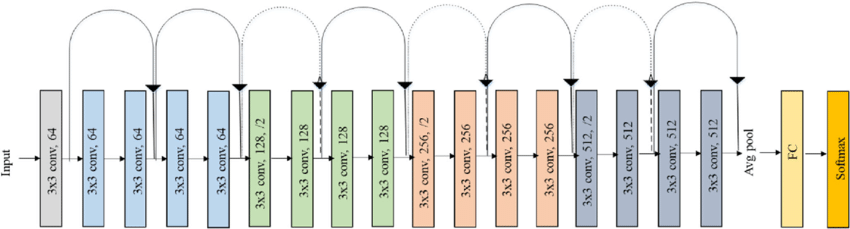
\includegraphics[width=0.9\textwidth]{images/ResNet-18-architecture.png}
    \captionof{figure}{ResNet-18 architecture. Figure taken from \cite{paper-with-resnet-18-figure}.
        The FC is short for Fully Connected layers, and the conv is short for convolutional layers. }
    \label{fig:resnet-18-architecture}
\end{center}


The architecture is implemented PyTorch\cite{PyTorch} and other similar libraries, making it easy to use.
